 \section{Actividad No 01 – DESARROLLO1} 
Ejercicio 1  Primeramente vamos conectar a datos existentes \\
	\begin{center}
	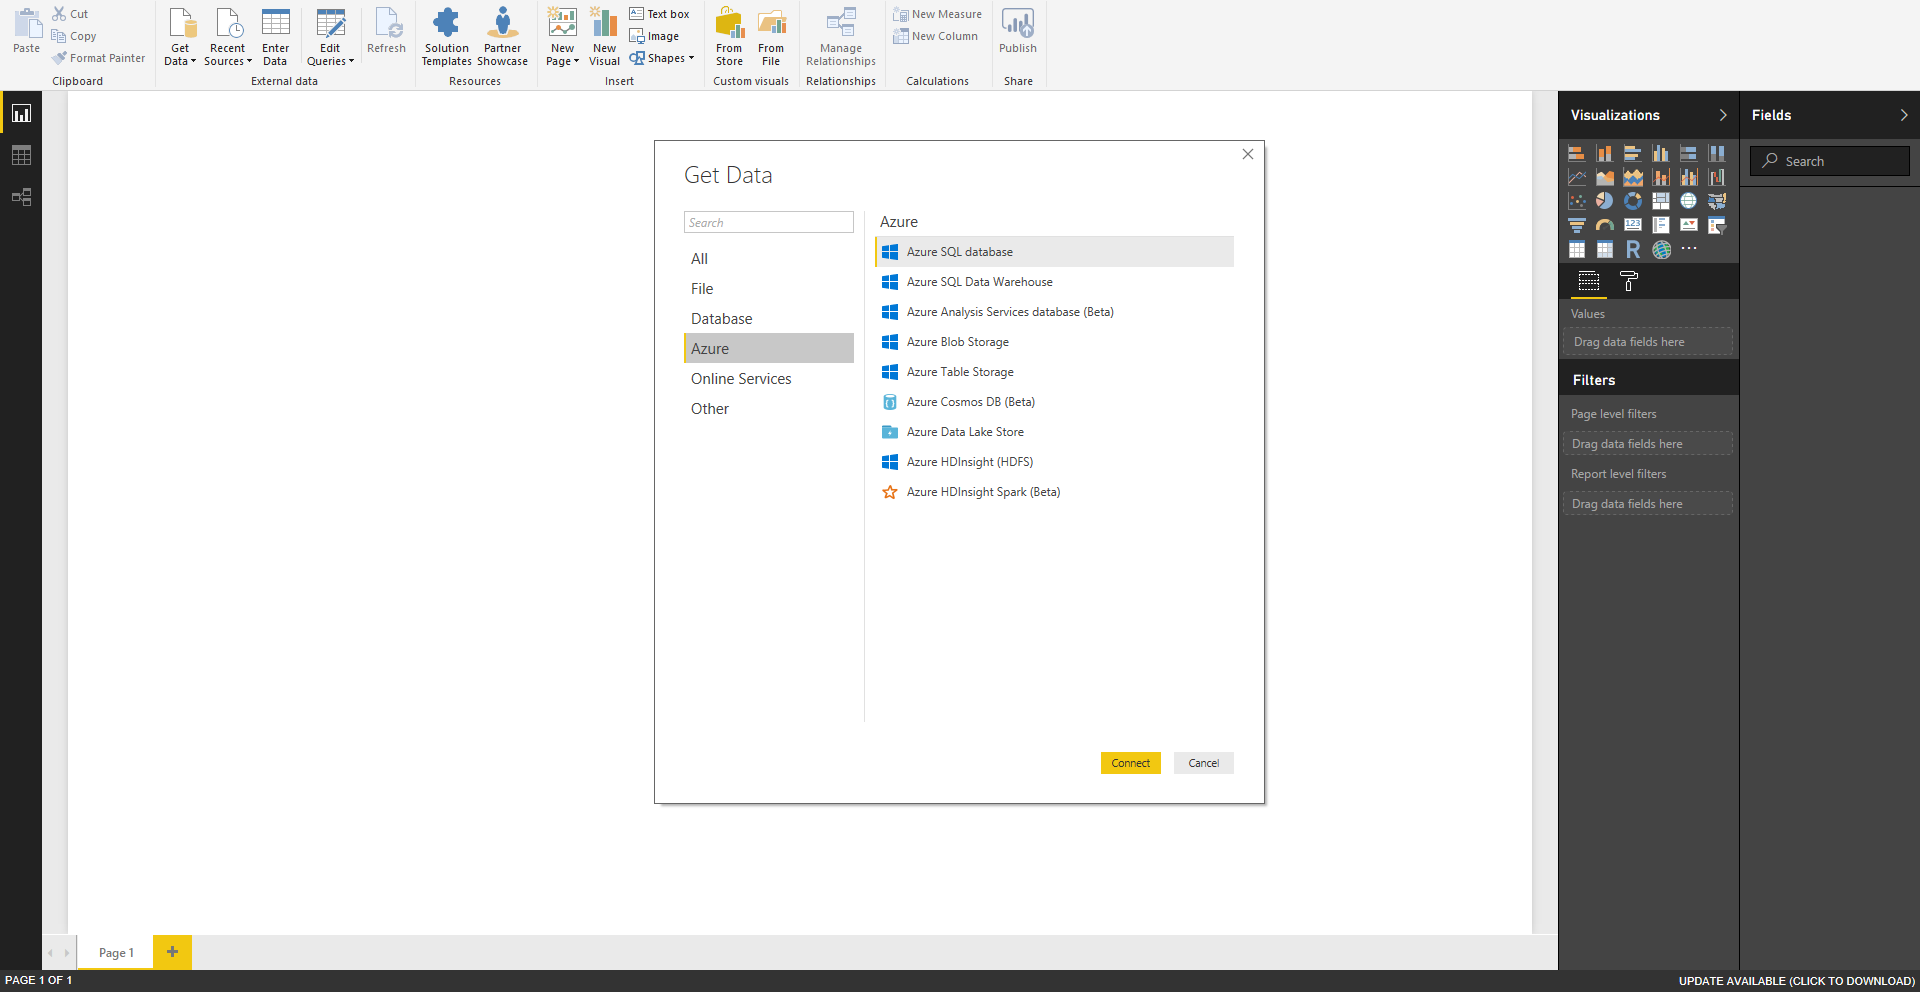
\includegraphics[width=15cm]{./Imagenes/Imagen1}
	\end{center}	

	\begin{center}
	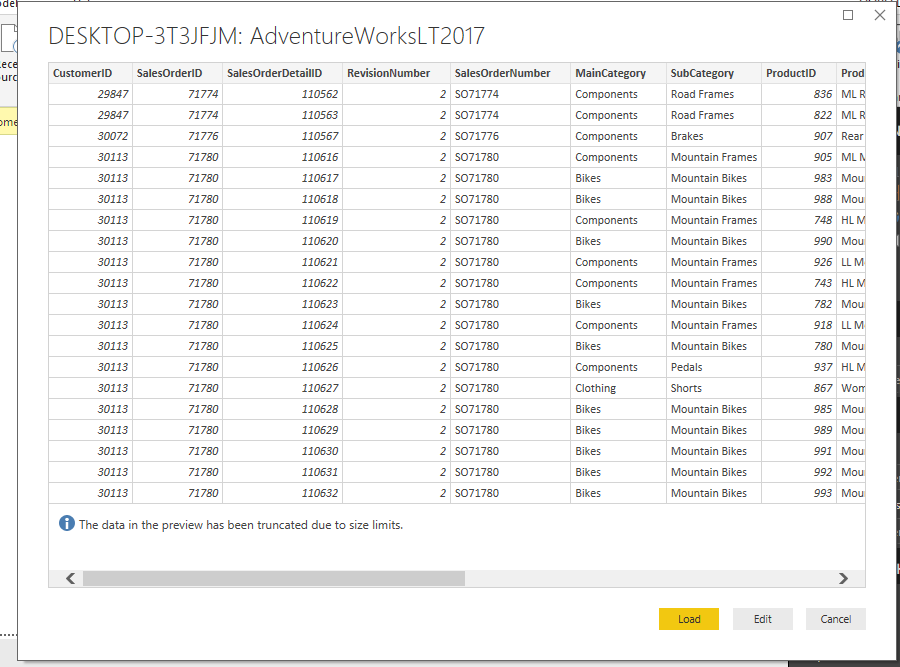
\includegraphics[width=15cm]{./Imagenes/Imagen2}
	\end{center}
	\newpage
	
Ejercicio 2: Seguidamente desarrollamos el Shape Data\\
	\begin{center}
	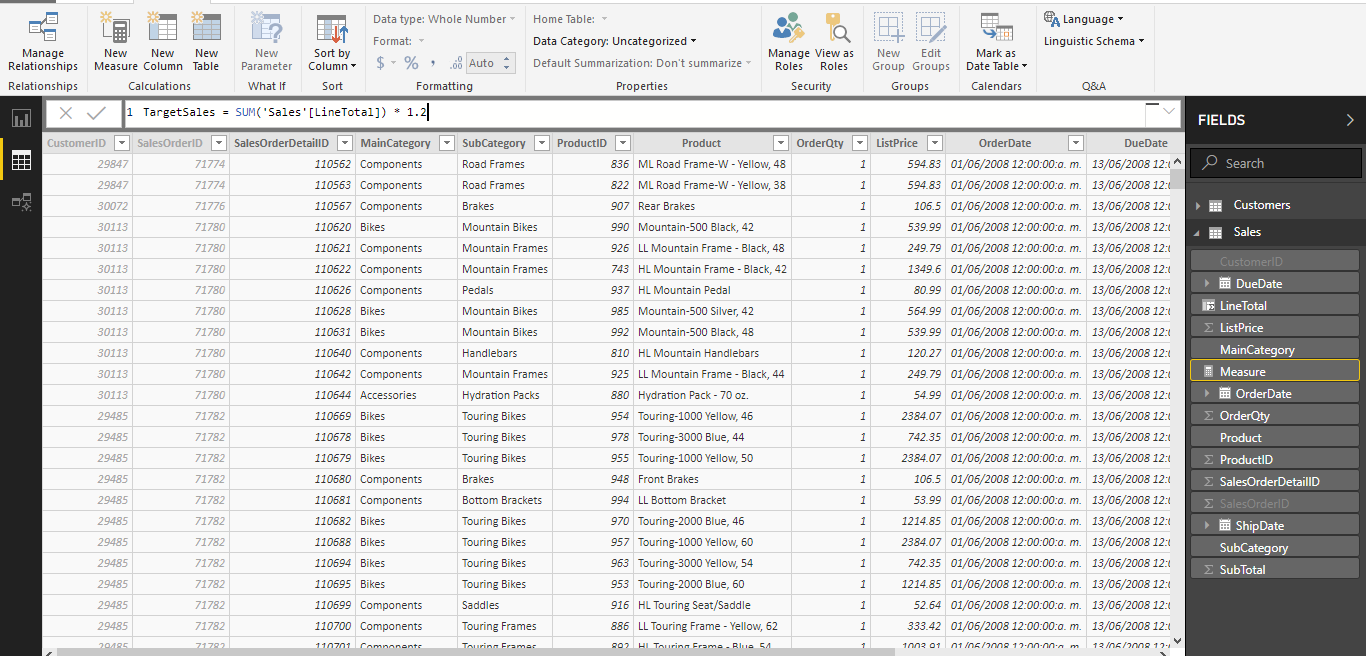
\includegraphics[width=15cm]{./Imagenes/Imagen3}
	\end{center}	

	

	\begin{center}
	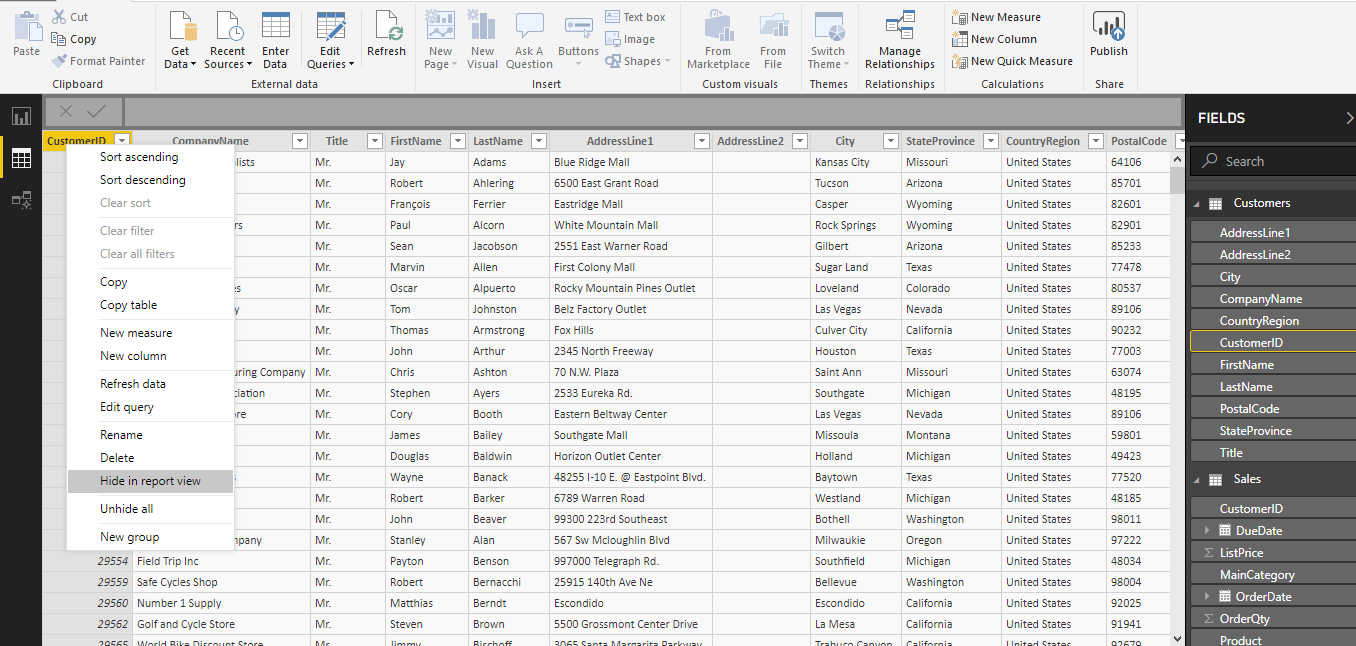
\includegraphics[width=15cm]{./Imagenes/Imagen4}
	\end{center}	
\newpage

	\begin{center}
	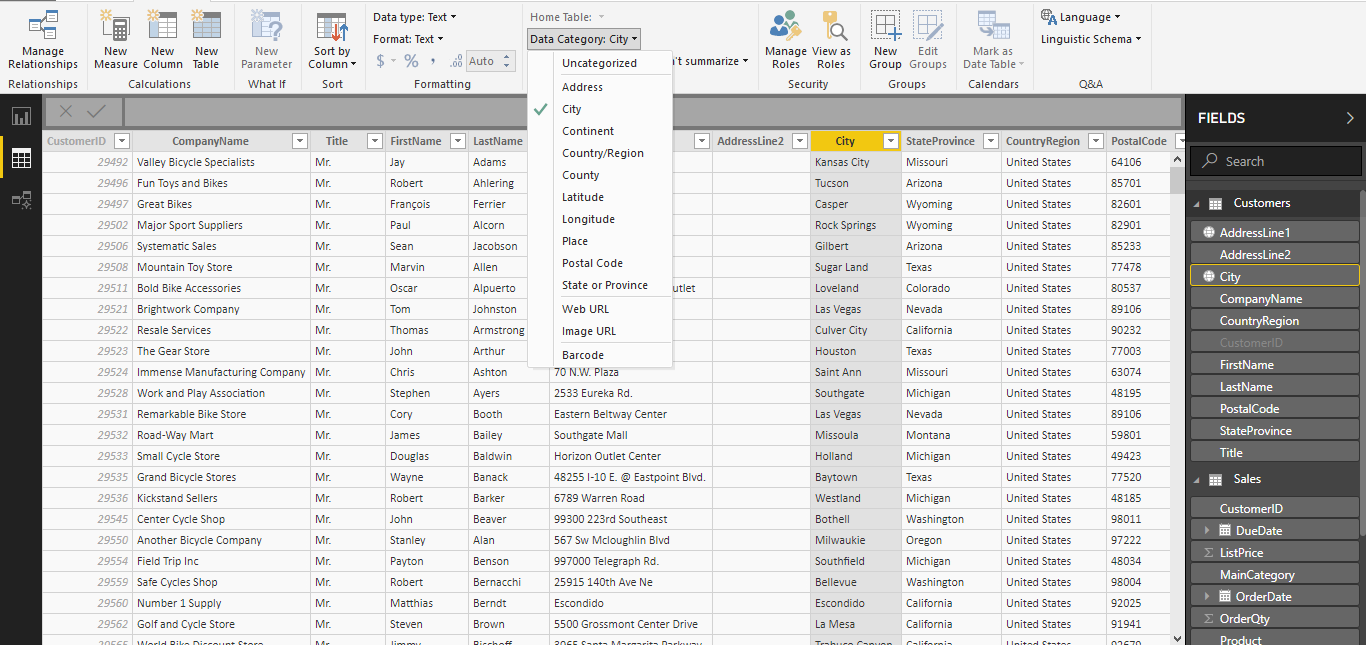
\includegraphics[width=15cm]{./Imagenes/Imagen5}
	\end{center}	

	\begin{center}
	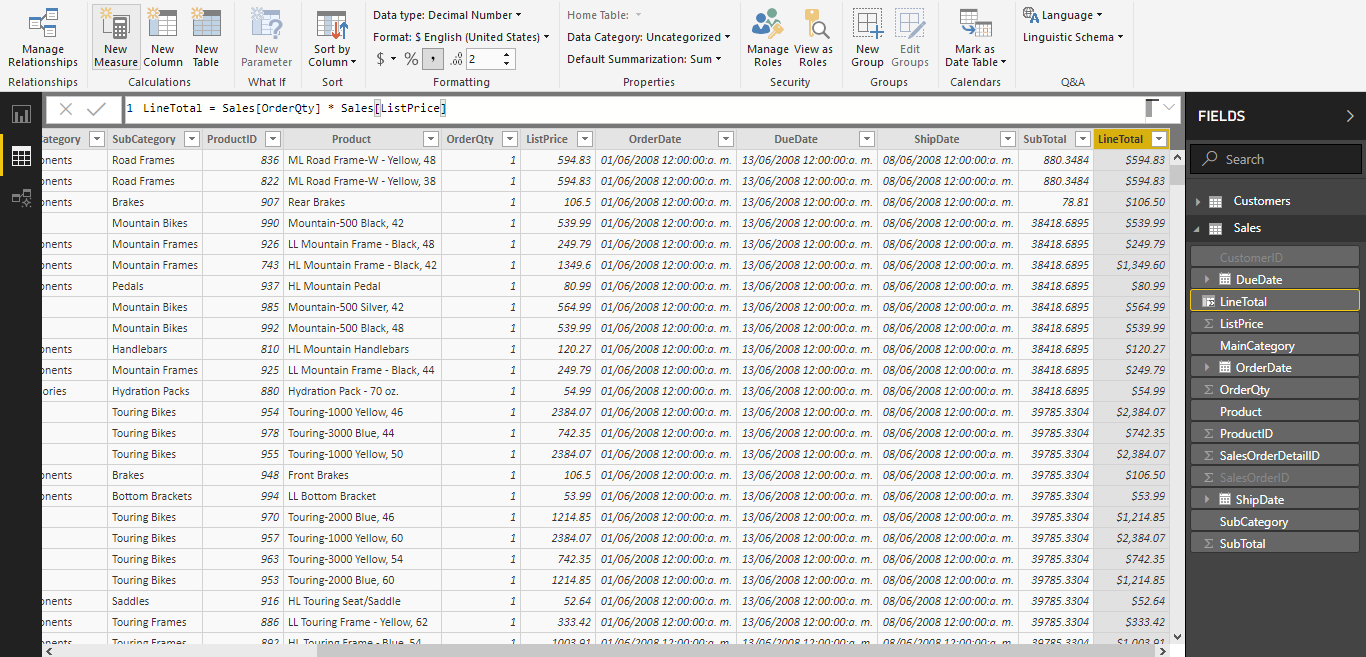
\includegraphics[width=15cm]{./Imagenes/Imagen6}
	\end{center}	
\newpage

Ejercicio 3: Ahora ahoramos la Combine Data\\
	\begin{center}
	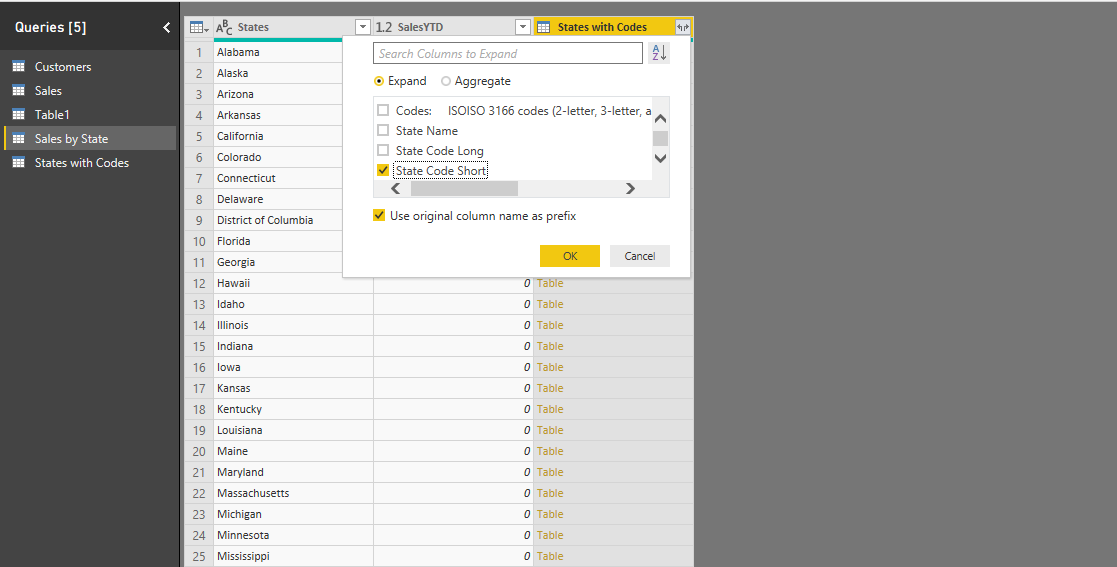
\includegraphics[width=15cm]{./Imagenes/Imagen7}
	\end{center}	

	\begin{center}
	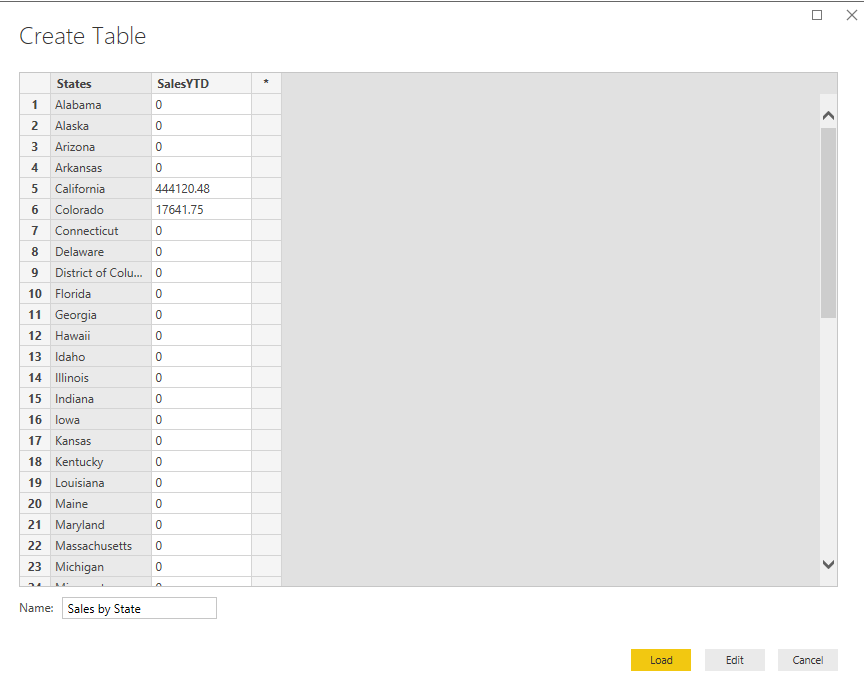
\includegraphics[width=15cm]{./Imagenes/Imagen8}
	\end{center}	
\newpage
	

	\begin{center}
	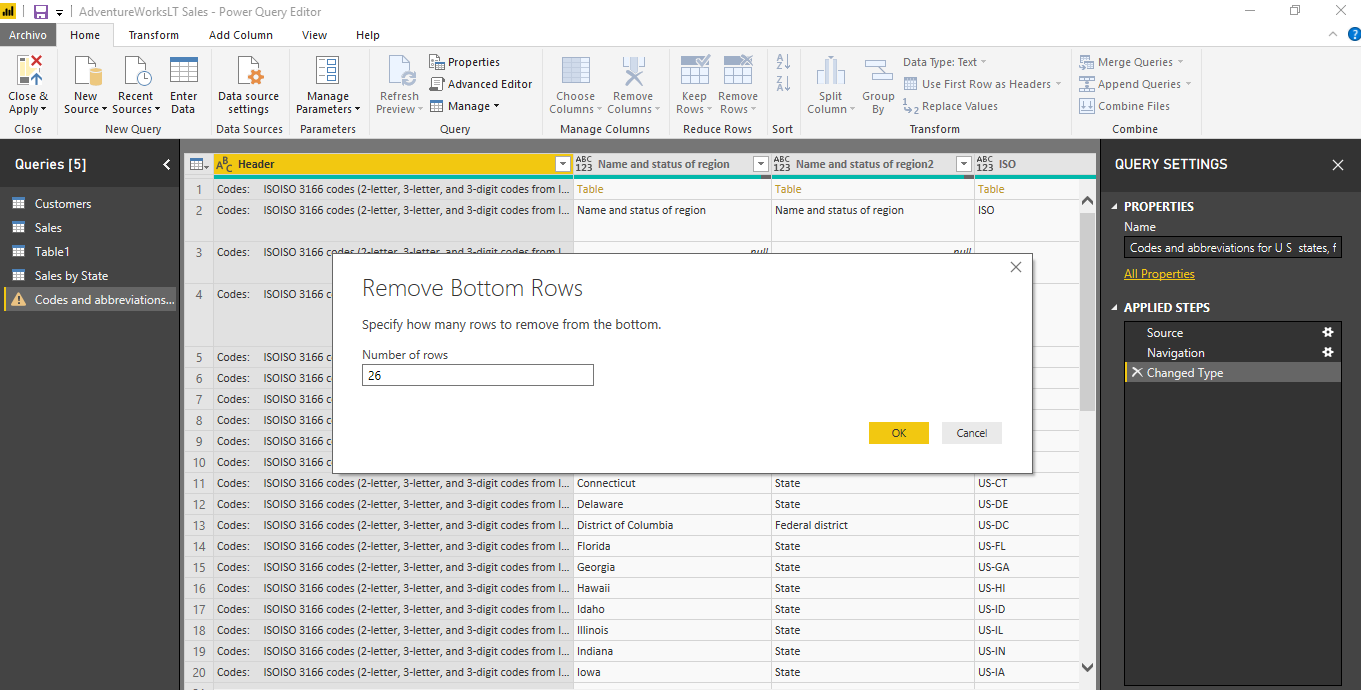
\includegraphics[width=15cm]{./Imagenes/Imagen9}
	\end{center}	
	

	\begin{center}
	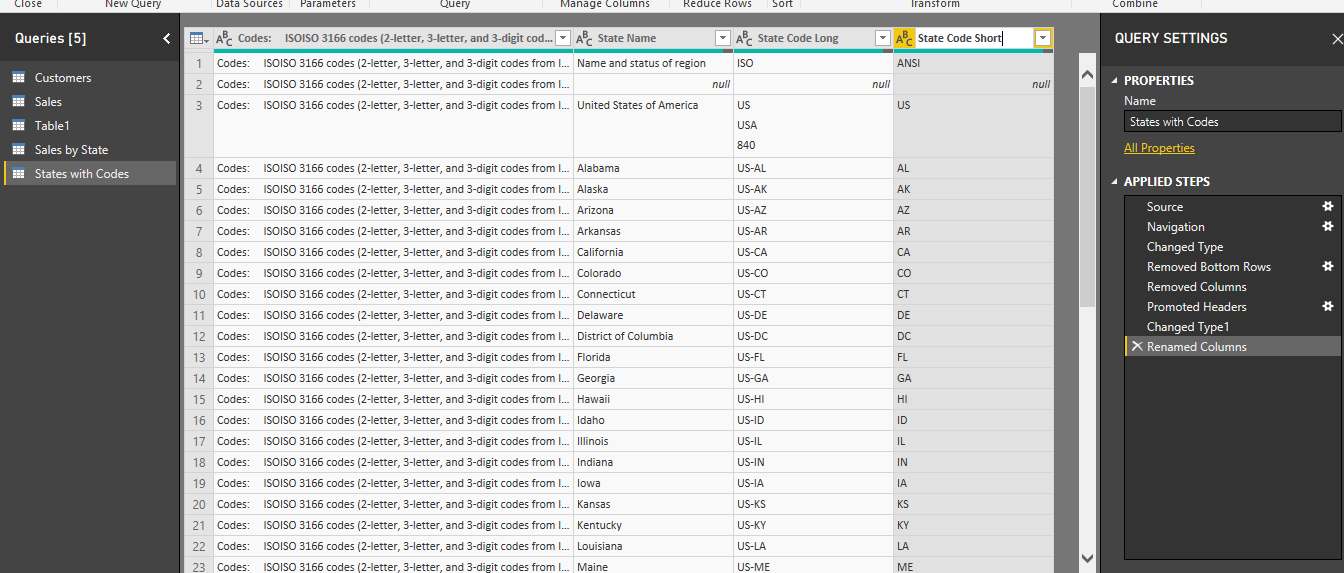
\includegraphics[width=15cm]{./Imagenes/Imagen10}
	\end{center}	
\newpage
	\begin{center}
	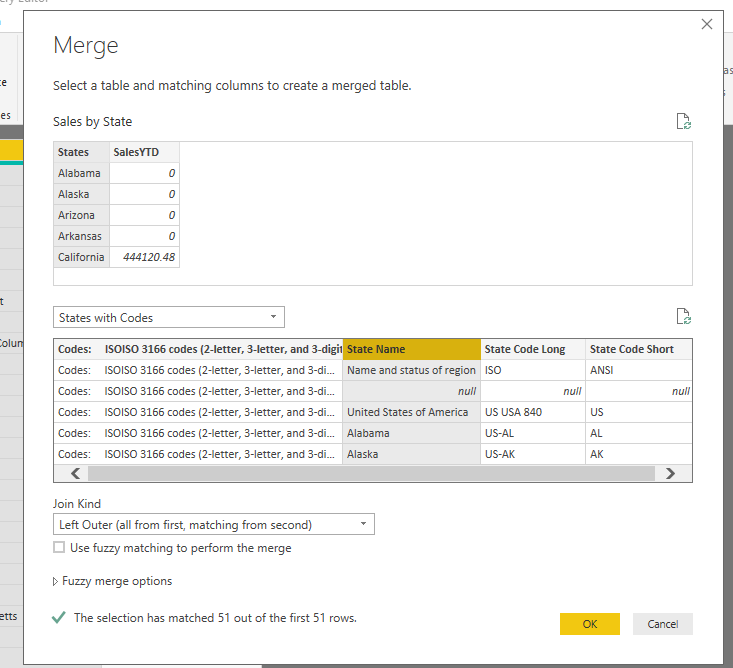
\includegraphics[width=15cm]{./Imagenes/Imagen11}
	\end{center}	


